% !TeX spellcheck = en_US

\chapter{Introduction}\label{chp:introduction}
\section{Intelligence Augmentation}
Periodically, cadastral survey data has to be updated. Generally spoken, this means among others to find changes in landcover based on aerial imagery (orthophotos, lidar, terrestrial measurements), which consists of new objects that have been added, existing objects that have changed or objects that have been removed in contrast to the latest survey data. As a result of this, this data has to be updated periodically, for example all one to five years, which results in a lot of manual work, as it is often not trivial to find the changes mentioned above.

One of the most time consuming parts of this work is to find the actual changes, for example a new built house or a garage that has been added to an already existing building. In general, this is a tedious and time consuming task, that can not easily be automated. Due to this, our intention is not to develop a fully automated method but instead to support the person who is doing this work with artificial intelligence, what is called intelligence augmentation \cite{Engelbart.1962} and is a rather old concept. However, as described in the previous chapter, the intention is to do intelligence augmentation using state of the art technologies.

To understand the difference between intelligence augmentation (IA) and artificial intelligence (AI) \autoref{fig:introduction:ia_vs_ai} shows some examples.

\begin{figure}[H]
    \centering
	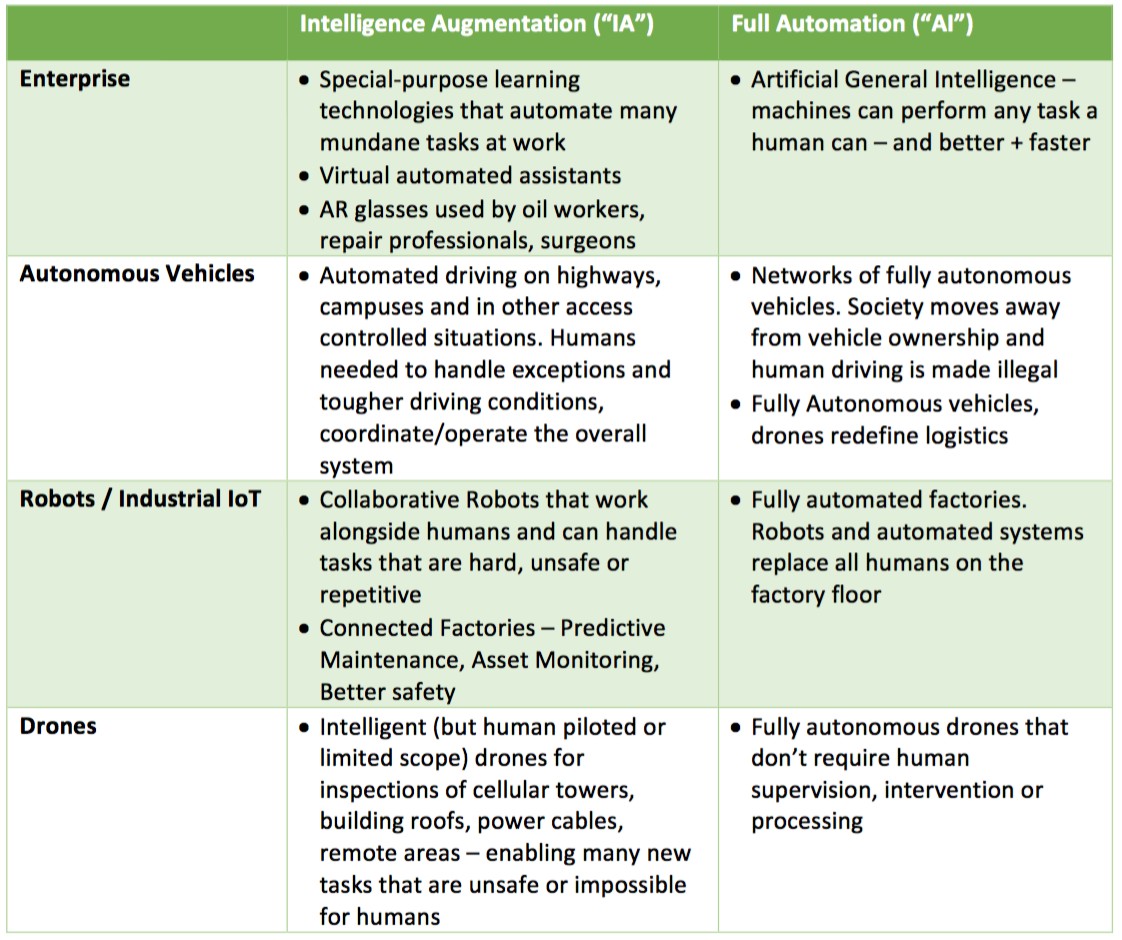
\includegraphics[width=0.9\linewidth]{chapters/introduction/images/ia_vs_ai.png}
	\caption{IA compared to AI\\Source: https://www.cbinsights.com/research/ai-vs-intelligence-augmentation-applications, 02.06.18}
	\label{fig:introduction:ia_vs_ai}
\end{figure}

\section{Architecture}
\autoref{fig:introduction:architecture_overview} shows an overview of the architecture. Note, that this diagram shows a combination of the learning and the prediction architecture. Step 2, which is loading the satellite imagery from Microsoft Bing is only required in the learning phase, that is for the generation of the training data, which is required to train the neural network.

\begin{figure}[H]
    \centering
	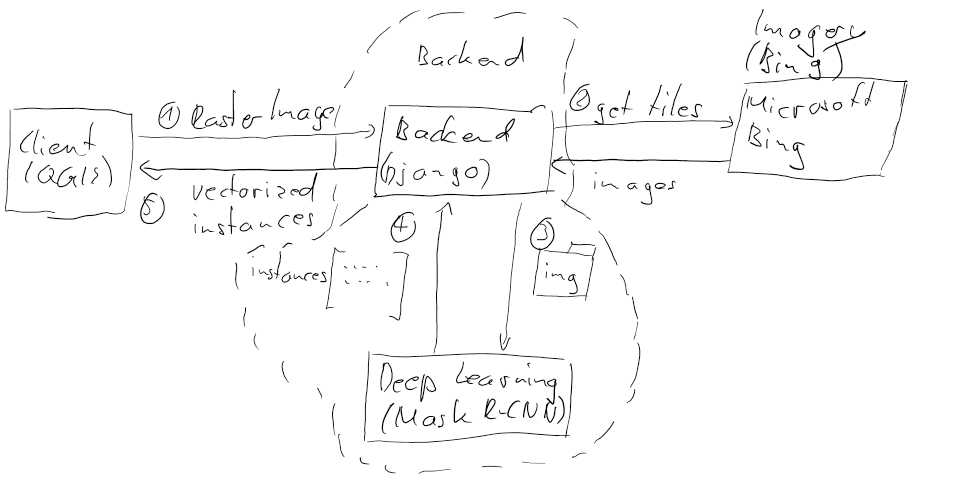
\includegraphics[width=0.9\linewidth]{chapters/introduction/images/overview.png}
	\caption{Architecture overview}
	\label{fig:introduction:architecture_overview}
\end{figure}

\autoref{fig:introduction:learning_phase} shows the data flow during the training of the neural network. For this step, satellite imagery from Microsoft Bing maps as well as OpenStreetMap (OSM) data is used. The satellite imagery is downloaded tile per tile for a predefined boundingn box and zoom-level and at the same time, binary images are created from the OSM data, which represent the ground truth. To simplify this step and make it available to the public, a tool called Airtiler \cite{airtiler} has been created and published.

\begin{figure}[H]
    \centering
	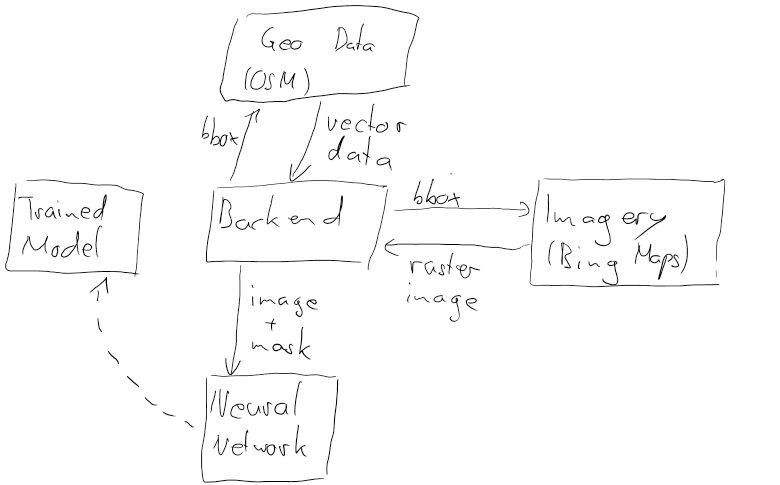
\includegraphics[width=0.9\linewidth]{chapters/introduction/images/learning_phase.png}
	\caption{Learning phase}
	\label{fig:introduction:learning_phase}
\end{figure}

As soon as the training is completed, the prediction can be done. For this thesis, this has been split into two phases. \autoref{fig:introduction:prediction_phase1} shows the data flow of phase 1, which passes the current extent as base64 encoded image data as well as the bounding box of the current QGIS extent to the configured backend webserver. The pretrained neural network is then used, to predict all instances on the current image. In the next step, the predicted instances are georeferenced using the boundingbox information that was sent to the backend at the beginning of the prediction phase. Finally, the georeferenced instances are sent back to the frontend client (the QGIS plugin), which then visualizes the data on a new layer in QGIS.

\begin{figure}[H]
    \centering
	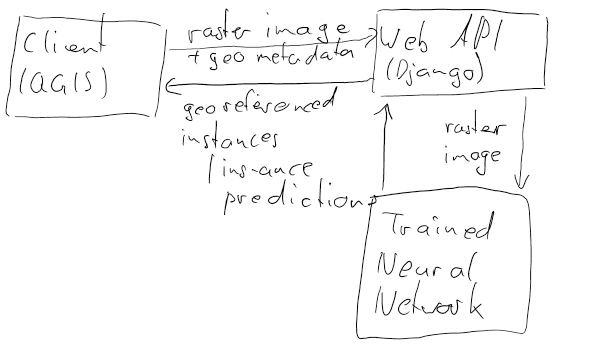
\includegraphics[width=0.9\linewidth]{chapters/introduction/images/inference_phase1.png}
	\caption{Prediction phase 1}
	\label{fig:introduction:prediction_phase1}
\end{figure}

\begin{figure}[H]
    \centering
	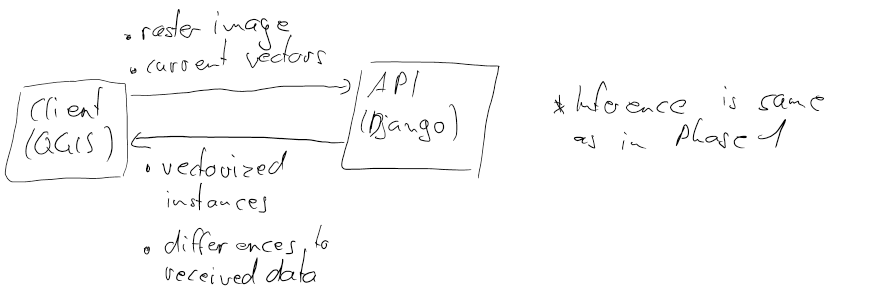
\includegraphics[width=0.9\linewidth]{chapters/introduction/images/inference_phase2.png}
	\caption{Prediction phase 2}
	\label{fig:introduction:prediction_phase2}
\end{figure}

\section{Hardware Requirements}
To train the neural network, a graphics card is required. We used a Nvidia P100 with 12 gigabytes of memory. A Nvidia GTX 750 was not sufficient due to only 2 gigabytes of memory. Additionally, CUDA\footnote{https://developer.nvidia.com/cuda-toolkit (22.06.18)} has to be installed aswell as Docker\footnote{https://www.docker.com/ (22.06.18)} and Nvidia-docker\footnote{https://github.com/NVIDIA/nvidia-docker (22.06.18)}.

How the docker image can be built and run is described in detail in the readme of the repository\footnote{https://github.com/mnboos/osm-instance-segmentation/blob/master/README.md (22.06.18)}.

\section{User Scenario}
This section describes a user scenario that can be used for example in a showcase or to instruct the actual end user on how to use the plugin with its corresponding backend. This user scenario requires, that the plugin is correctly installed in QGIS and the backend has been configured correctly in the settings of the plugin. Additionally, the backend has to be running.

\begin{enumerate}
    \item Start QGIS
    \item Load the data of the cadastral survey data. This may for example be a zip archive containing shape files according to the MOpublic \cite{mopublic}  specification. In this case, the archive can simply be dragged and dropped into QGIS. Followingly, a dialog will open which allows the select several layers. 
    \item Select the layers containing buildings and / or other geometries. Typically and according to MOpublic this layer is named \textit{BB\_BoFlaeche}.
    \item Load an imagery layer, for example Bing maps or Google maps. This can be done easily using the QGIS plugin \textit{OpenLayers}.
\end{enumerate}